\documentclass[a4paper,10pt]{article}
\usepackage[utf8]{inputenc}
 
% Blank line between paragraphs instead of indenting the first line
\usepackage{parskip}
\setlength{\parskip}{\baselineskip}

% Squash a bit more text onto a page
\usepackage{geometry}
\geometry{verbose,tmargin=20mm,bmargin=20mm,lmargin=20mm,rmargin=20mm}

\usepackage{graphicx}
\usepackage{listings}
\usepackage{amsmath}
\usepackage{color}
\usepackage{dirtree}
\usepackage{verbatim}

% Indent verbatim environments
\makeatletter \def\verbatim@processline{\hspace*{2em}\the\verbatim@line\par}\makeatother

\definecolor{mygreen}{rgb}{0,0.6,0}
\definecolor{mygray}{rgb}{0.5,0.5,0.5}
\definecolor{mymauve}{rgb}{0.58,0,0.82}

\lstset { 
  backgroundcolor=\color{white},   % choose the background color; you must add \usepackage{color} or \usepackage{xcolor}
  basicstyle=\footnotesize,        % the size of the fonts that are used for the code
  breakatwhitespace=false,         % sets if automatic breaks should only happen at whitespace
  breaklines=true,                 % sets automatic line breaking
  captionpos=b,                    % sets the caption-position to bottom
  commentstyle=\color{mygreen},    % comment style
  deletekeywords={...},            % if you want to delete keywords from the given language
  escapeinside={\%*}{*)},          % if you want to add LaTeX within your code
  extendedchars=true,              % lets you use non-ASCII characters; for 8-bits encodings only, does not work with UTF-8
  frame=single,                    % adds a frame around the code
  keepspaces=true,                 % keeps spaces in text, useful for keeping indentation of code (possibly needs columns=flexible)
  keywordstyle=\color{blue},       % keyword style
  language=C++,                    % the language of the code
  morekeywords={*,DEVICES,
  				CONNECTIONS,
  				MONITORS,
  				END}, 	           % if you want to add more keywords to the set
  numbers=left,                    % where to put the line-numbers; possible values are (none, left, right)
  numbersep=5pt,                   % how far the line-numbers are from the code
  numberstyle=\tiny\color{mygray}, % the style that is used for the line-numbers
  rulecolor=\color{black},         % if not set, the frame-color may be changed on line-breaks within not-black text (e.g. comments (green here))
  showspaces=false,                % show spaces everywhere adding particular underscores; it overrides 'showstringspaces'
  showstringspaces=false,          % underline spaces within strings only
  showtabs=false,                  % show tabs within strings adding particular underscores
  stepnumber=1,                    % the step between two line-numbers. If it's 1, each line will be numbered
  stringstyle=\color{mymauve},     % string literal style
  tabsize=2,                       % sets default tabsize to 2 spaces
  title=\lstname                   % show the filename of files included with \lstinputlisting; also try caption instead of title
}

\begin{document}
%\contentsname{IIA GF2 Software: Final Report}
\begin{center}
\Huge \textbf{IIA GF2 Software: Final Report}

\large Jamie Magee (jam96) \\ Team 8 \\ Gonville \& Caius College
\end{center}

\tableofcontents
\pagebreak

\section{Description}
Our logic simulator is able to simulate any number of circuits which include the following devices:

\begin{itemize}
\item Clocks
\item Switches
\item AND gates (Up to 16 inputs)
\item NAND gates (Up to 16 inputs)
\item OR gates (Up to 16 inputs)
\item NOR gates (Up to 16 inputs)
\item XOR gates
\item D-Type flip-flops
\item Signal generators
\end{itemize}

It uses files written in the language as specified in our EBNF in Appendix~\ref{sec:EBNF}, with the file extension \texttt{.gf2} and have MIME type \texttt{text/plain}. Errors in a definition file are reported fully to the user upon reading a definition file, and give unique error codes for each different type of error. There is no limit on the number of devices in a network (except for that implied by the available memory of the computer). There may also be an unlimited number of monitors. For a complete guide on how to operate our logic simulator, please see the user guide in Appendix~\ref{sec:guide}.

For the structure of our logic simulator we made use of modularisation through the use of object oriented programming. The logic circuit is internally represented using the network class, in addition to the devices class which stores details about the properties of each device. Names of devices are represented internally by a unique integer. The names class handles the storage of names as they are read in, as well as storing a list of reserved names upon instantiation. When a file is opened, it is read by the parser class, by creating an instance of the scanner class which reads through the definition file character, by character, building them up into symbols which are returned to the parser. Depending on the order of the symbols that were read in, the parser can create devices, connections or monitors (or throw errors). Once the entire definition file has been read in, the gui class interprets commands issued by the user and makes appropriate calls to the network, monitor and devices classes. 

\section{Development Style}

We split the development of our logic simulator into five major phases: specification, design, implementation, testing and maintenance. The timeframe was then decided for each task and each task was assigned to either a team member or the whole team, depending on the nature of the task. A Gantt chart showing our time planning can be seen in Appendix~\ref{sec:gantt}.

Each member of the team was also assigned a general project role as follows:

\textbf{Project manager:} (T Hillel) - Responsible for project planning including delegation of tasks and ensuring that the project runs to the set timescale.

\textbf{Programming administrator:} (J Magee) - Responsible for upkeep of the project directory including performing builds and keeping legacy versions of the simulator.

\textbf{Client representative:} (M Jackson) - Responsible for ensuring that the project meets the client's requirements for the logic simulator as defined in Appendix A of the GF2 Project Handout.

We made significant use of \texttt{git} for revision control, as well as GitHub for tracking bugs in the software and features required by the client. It also allowed us to work on the same file independently and merge our changes using the \texttt{git merge} command.

During the maintenance phase of the project we divided up the tasks and tackled them independently. They were assigned as follows:

\textbf{Non-zero Hold Time of Bistables:} J Magee

\textbf{Signal Generators:} T Hillel

\textbf{Continuous Simulation:} M Jackson

While the tasks were split up, and the person assigned to the task contributed the majority of the code, the power of \texttt{git} allowed other members of the team to contribute easily.

Overall I believe our team worked efficiently, and as a result we were able to achieve all the requirements of the client within the deadlines we were set.

\section{My Contribution}

I took on responsibility for writing the names and scanner classes. In addition, I wrote approximately 25\% of the parser class. the names class stores a list of all the words used within a definition file, and methods to manipulate them. It is initialised with only the reserved words, but can be populated as a definition file is read. the scanner class reads through the definition file, character by character, and is able to return complete symbols to the parser. It is able to return the internal representation of a symbol, the type of symbol and optionally the value. The parser class analyses the definition file as it is read in according to the rules laid out in our EBNF. It is then able to create devices, connections and monitors that are laid out in the definition file. I wrote the \texttt{newConnection, monitorList} and \texttt{newMonitor} methods. The \texttt{newConnection} and \texttt{newMonitor} methods deal with reading in a connection and monitor respectively, and creating them using the network and monitor classes respectively. The \texttt{monitorList} class deals with reading in an entire \texttt{MONITOR} block, as defined by our EBNF, which can be seen in Appendix~\ref{sec:EBNF}

Once the majority of the software was written, I designed a definition file for each error and warning our logic simulator can throw and then wrote a shell script which would attempt to run each definition file, and record the output from our logic simulator. In addition to testing for errors, I wrote a shell script which would run through each of our test definition files, in Appendix~\ref{sec:examples}, and record the output. Both the shell scripts can be found in Appendix~\ref{sec:tests}.

During the maintenance phase of the project, I undertook the task to implement a non-zero hold time for d-type flip flops, as well as randomising the order of execution of devices. the non-deterministic characteristics of d-types required editing of the devices class, specifically the \texttt{execdtype} method. Randomising the order of execution of devices was implemented in the network class, and required reading the values from the existing devices list, shuffling the list (while still retaining clocks at the end of the list) and writing it back.

\section{Testing}

We used two main tests of testing - unit and system testing - both of which are industry standard practices. For our unit testing, Martin wrote an errors class which compared the actual output from various units of code, to the expected output. For system testing I wrote a shell script which passed definition files to the logic simulator and recorded the output in a text file. There were two variations on the shell script: One which ran known good definition files and therefore had to input the commands to run the simulation in addition to recording the output; Another which ran known bad definition files and only expected parsing errors which it recorded. An example of the output produced by the the test shell script is as follows:
\pagebreak
\begin{verbatim}
processing sipo.gf2...
Logic Simulator: interactive command interface
# Running for 50 cycles
CLK2               :_-_-_-_-_-_-_-_-_-_-_-_-_-_-_-_-_-_-_-_-_-_-_-_-_-
D1.Q               :___--__--__--__--__--__--__--__--__--__--__--__--_
D2.Q               :_____--__--__--__--__--__--__--__--__--__--__--__-
D3.Q               :_______--__--__--__--__--__--__--__--__--__--__--_
D4.Q               :_________--__--__--__--__--__--__--__--__--__--__-
# Logic Simulator: terminating.
\end{verbatim}

An example of the output produced by the error shell script is as follows:

\begin{verbatim}
processing 12.gf2...
Line 11:
1.I1 = S1;
^
Error 0x000C: Connection must start with the name of a device
Unconnected Input : G1.I1
There is 1 error
\end{verbatim}


\section{Conclusions}

Overall I believe that we worked well as a team, and were able to achieve the requirements set out by the client. We made effective use of \texttt{git} for revision control, bug tracking and feature requests. This allowed us to focus more on writing code, and less time on code management. Due to our extensive tests - both unit and system - we were able to quickly identify bugs in our code before committing them to our GitHub repository. This again, allowed more time to be spent on writing code, and less time hunting down bugs. 

If we had more time I would improve our logic simulator by:

\begin{itemize}
\item Implementing a WYSIWYG GUI
\item Improving the parser to allow simple error correction
\item Expand the device library to include JK flip-flops and XNOR gates
\item Rearrange monitors in the GUI by dragging and dropping
\item Save changes made to a circuit using the GUI, to the definition file
\item Export the monitors from the GUI to CSV or PNG
\end{itemize}

\pagebreak

\appendix
\section{Code Listings}
\subsection{Names Class}
\subsubsection{names.h}
\lstinputlisting[caption=names.h]{../../src/names.h}
\subsubsection{names.cc}
\lstinputlisting[caption=names.cc]{../../src/names.cc}

\subsection{Scanner Class}
\subsubsection{scanner.h}
\lstinputlisting[caption=scanner.h]{../../src/scanner.h}
\subsubsection{scanner.cc}
\lstinputlisting[caption=scanner.cc]{../../src/scanner.cc}

\subsection{Parser Class}
\subsubsection{parser.cc}
\lstinputlisting[caption=parser.cc]{../../src/parser.cc}

\texttt{parser.cc} was written with joint effort between myself and Tim. I contributed approximately 25\% of the code.

\subsection{Test Scripts}
\label{sec:tests}
\subsubsection{test.sh}
\lstinputlisting[caption=test.sh,language=bash,label=test-script]{../../examples/test.sh}
\subsubsection{error.sh}
\lstinputlisting[caption=error.sh,language=bash]{../../examples/errors/error.sh}
\pagebreak

\section{Test Definition Files}
\label{sec:examples}

All supplied definition files and circuit diagrams were written and designed by myself.

\subsection{XOR Gate}

\subsubsection{Definition File}
\lstinputlisting[caption=xor.gf2]{../../examples/xor.gf2}

\subsubsection{Circuit Diagram}
\begin{figure}[h]
 \centering
 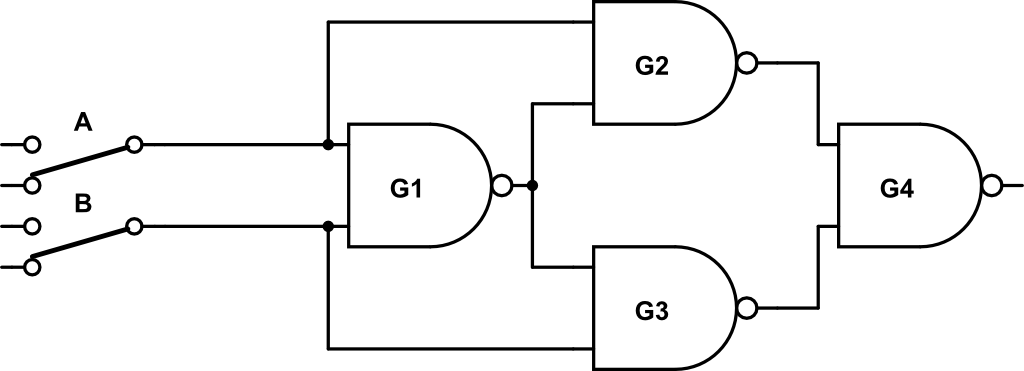
\includegraphics[width=8cm]{../../examples/xor.png}
 \caption{Circuit diagram of an XOR gate implemented using NAND gates}
 \label{fig:example-xor}
\end{figure}

\subsection{4-bit Adder}

\subsubsection{Definition File}
\lstinputlisting[caption=4bitadder.gf2]{../../examples/4bitadder.gf2}

\subsubsection{Circuit Diagram}
\begin{figure}[h]
 \centering
 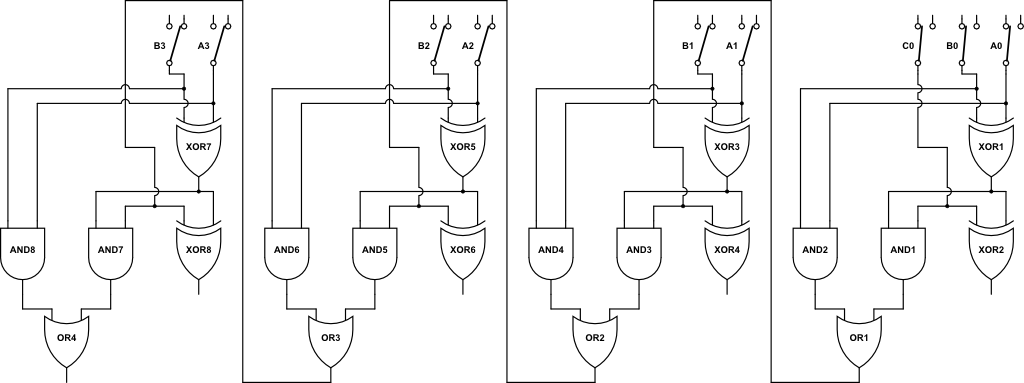
\includegraphics[width=14cm]{../../examples/4-bit-adder.png}
 \caption{Circuit diagram of a 4-bit adder}
 \label{fig:example-adder}
\end{figure}

\subsection{Serial In Parallel Out Shift Register}

\subsubsection{Definition File}
\lstinputlisting[caption=sipo.gf2]{../../examples/sipo.gf2}

\subsubsection{Circuit Diagram}
\begin{figure}[h]
 \centering
 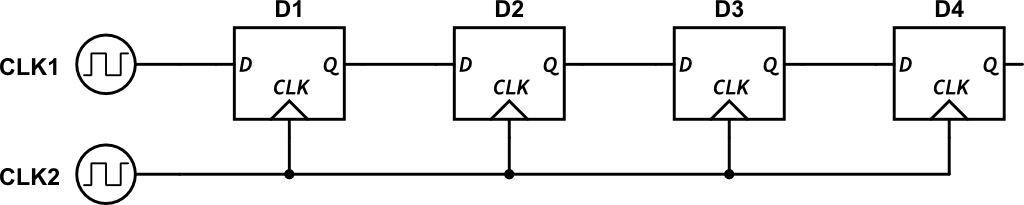
\includegraphics[width=12cm]{../../examples/sipo.png}
 \caption{Circuit diagram of a serial in parallel out shift register}
 \label{fig:example-sipo}
\end{figure}

\textbf{NB} The software used to draw the circuit diagram does not support the same style of D flip-flop used in the definition file, and Fig. \ref{fig:example-sipo} was the closest achievable.

\subsection{Gated D Latch}

\subsubsection{Definition File}
\lstinputlisting[caption=sipo.gf2]{../../examples/gateddlatch.gf2}

\subsubsection{Circuit Diagram}
\begin{figure}[h]
 \centering
 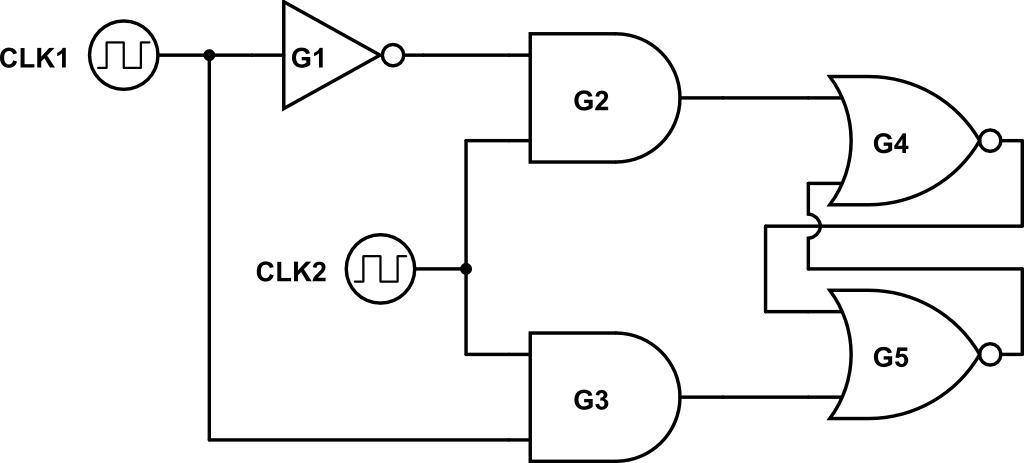
\includegraphics[width=9cm]{../../examples/gated-d-latch.png}
 \caption{Circuit diagram of a Gated D Latch}
 \label{fig:example-dlatch}
\end{figure}

\textbf{NB} The software used to draw the circuit diagram does not support the NAND gates with one input. Therefore the NAND gate G1 was substituted for a NOT gate as can be seen in Fig. \ref{fig:example-dlatch}.

\subsection{Signal Generator Example}

\subsubsection{Definition File}
\lstinputlisting[caption=siggen.gf2]{../../examples/siggen.gf2}

\subsubsection{Circuit Diagram}
\begin{figure}[h]
 \centering
 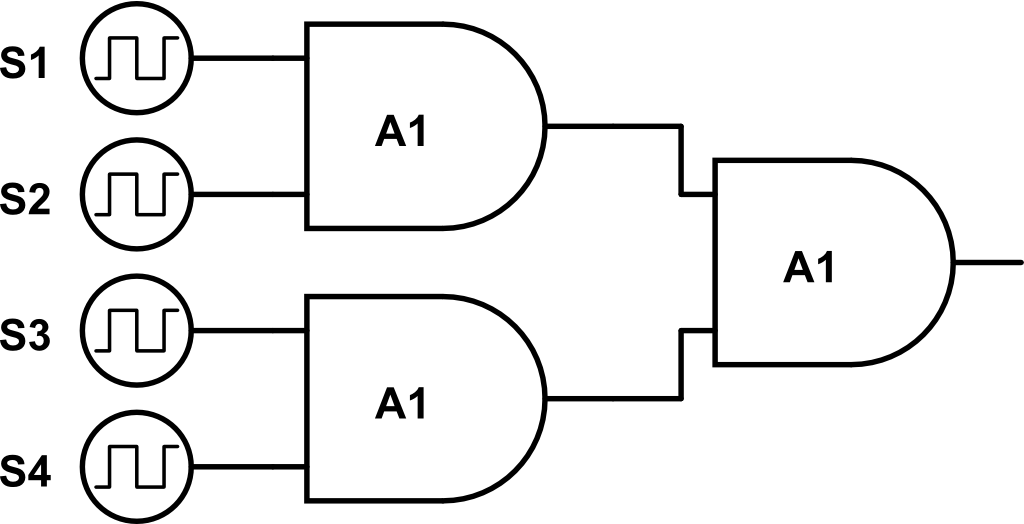
\includegraphics[width=9cm]{../../examples/siggen.png}
 \caption{Circuit diagram using a signal generator}
 \label{fig:example-siggen}
\end{figure}

\textbf{NB} The software used to draw the circuit diagram does not support the AND gates with four inputs. Therefore three AND gates with two inputs each were substituted for the single AND gate, A1, with four inputs as can be seen in Fig. \ref{fig:example-siggen}.

\pagebreak

\section{EBNF}
\label{sec:EBNF}
\lstinputlisting[caption=EBNF, language=python]{../../docs/ebnf.txt} %python seems to work okay

\pagebreak

\section{User Guide}
\label{sec:guide}

\textbf{Opening files:} To open a definition file, click the \texttt{File} menu followed by the \texttt{Open} option. You will be presented with a file selection dialogue. The file selection dialogue will only show definition files (Files with the \texttt{.gf2} file extension). Upon selecting a file, any errors in the definition file will be written to the message window, otherwise the Logic Simulator is ready to use. 

\begin{figure}[h]
        \centering
        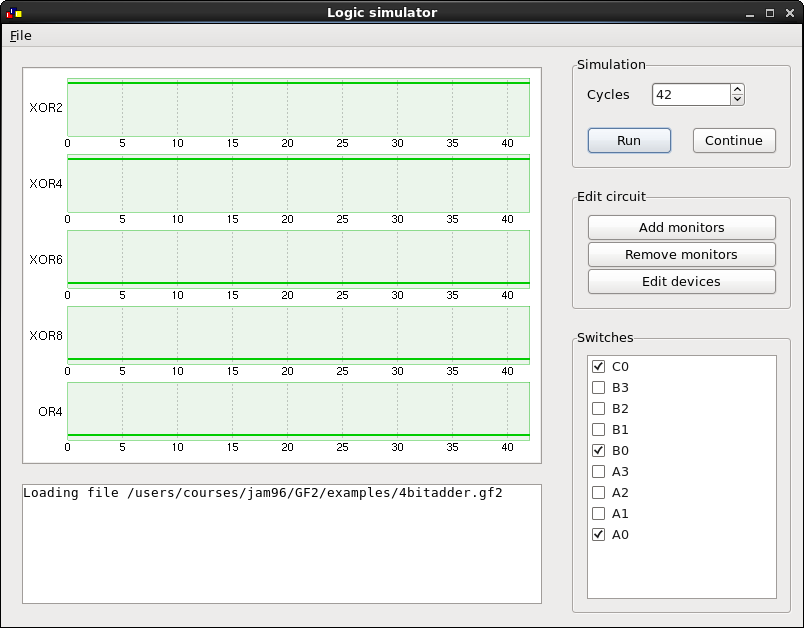
\includegraphics[width=.8\textwidth]{../../report2/jam96/simulation}
        \caption{The view upon running a simulation}
        \label{fig:simulation}
\end{figure}

\textbf{Running simulations:} In order to run a simulation you must first enter a number of cycles you wish the simulation to run for (default is \texttt{10}) then press the run button. The monitored signals will be displayed in the left display panel. You may choose to continue the simulation by pressing the \texttt{Continue} button, or run the simulation continuously by pressing the \texttt{Continuous Simulation} button.

\textbf{Adding or removing monitors:} You can edit the signals that are monitored and displayed in the main window. To add monitors, click the \texttt{Add monitors} button and select the monitor, or monitors, you wish to add followed by the \texttt{OK} button. To remove monitors, press the \texttt{Remove monitors} button and select the monitor, or monitors, you wish to remove followed by the \texttt{OK} button

\textbf{Editing devices:} To edit devices, click the \texttt{Edit devices} button. From the Edit devices dialogue you can change the device's name, type and number of inputs (if applicable). You can also change the inputs to, or ouputs from a device.

\textbf{Changing switch states:} If your circuit contains any  switches, you can change the state of the switch by changing the state of the check box beside its name.

\textbf{Changing simulator settings:} You can change certain settings relating to the operation of the logic simulator. Click the \texttt{Options} menu and from here you can change or reset settings as well as adjust the continuous run speed. By clicking \texttt{Edit options} you can change the trace options and debugging options.


\pagebreak

\section{File Listing}
\setlength{\DTbaselineskip}{15pt}
\DTsetlength{.2em}{3em}{0.1em}{1pt}{4pt}
\dirtree{.1 logsim.
.2 docs.
.2 examples.
.3 errors.
.2 report1.
.2 report2.
.2 report3.
.2 src.
.3 names.*.
.3 scanner.*.
.3 parser.*.
.3 devices.*.
.3 network.*.
.3 monitor.*.
.3 gui.*.
.3 logsim.*.
}

\textbf{docs} contains documentation relevant to our logic simulator such as: EBNF, reserved words, and our Gantt chart.

\textbf{examples} contains our example definition files as listed in Appendix~\ref{sec:examples} as well as the test shell script listed in Appendix~\ref{sec:tests}.

\textbf{errors} contains definition files which contain deliberate errors and are used to test our error checking functionality. In addition this folder contains the error.sh shell script listed in Appendix~\ref{sec:tests}.

\textbf{report1, report2} and \textbf{report3} contain our first, second and final report respectively.

\textbf{src} contains the source code for our logic simulator. The functionality of the major classes is outlined beneath.

\textbf{names} stores a list of all the words used within a definition file, and methods to manipulate them. It is initialised with only the reserved words, but can be populated as a definition file is read.

\textbf{scanner} reads through the definition file, character by character, and is able to return complete symbols to the parser. It is able to return the internal representation of a symbol, the type of symbol and optionally the value.

\textbf{parser} analyses the definition file as it is read in according to the rules laid out in our EBNF. It is then able to create devices, connections and monitors that are laid out in the definition file.

\textbf{devices} is used to create and execute devices. 

\textbf{network} stores information about the devices, including the connections between each device.

\textbf{monitor} implements signal monitors, which are used to display the points of interest, as determined from the definition file, in the GUI.

\textbf{gui} provides a graphical user interface for the user, and allows for advanced features such as circuit and monitor editing without having to edit the definition file. We have implemented the GUI with a modular approach, and as such there are several gui related classes e.g. gui-canvas, gui-id, gui-misc, etc.

\textbf{logsim} ties all the other classes together and allows the user to fully simulate logic circuits.

\pagebreak

\section{Gantt Chart}
\label{sec:gantt}

\begin{figure}[h]
 \centering
  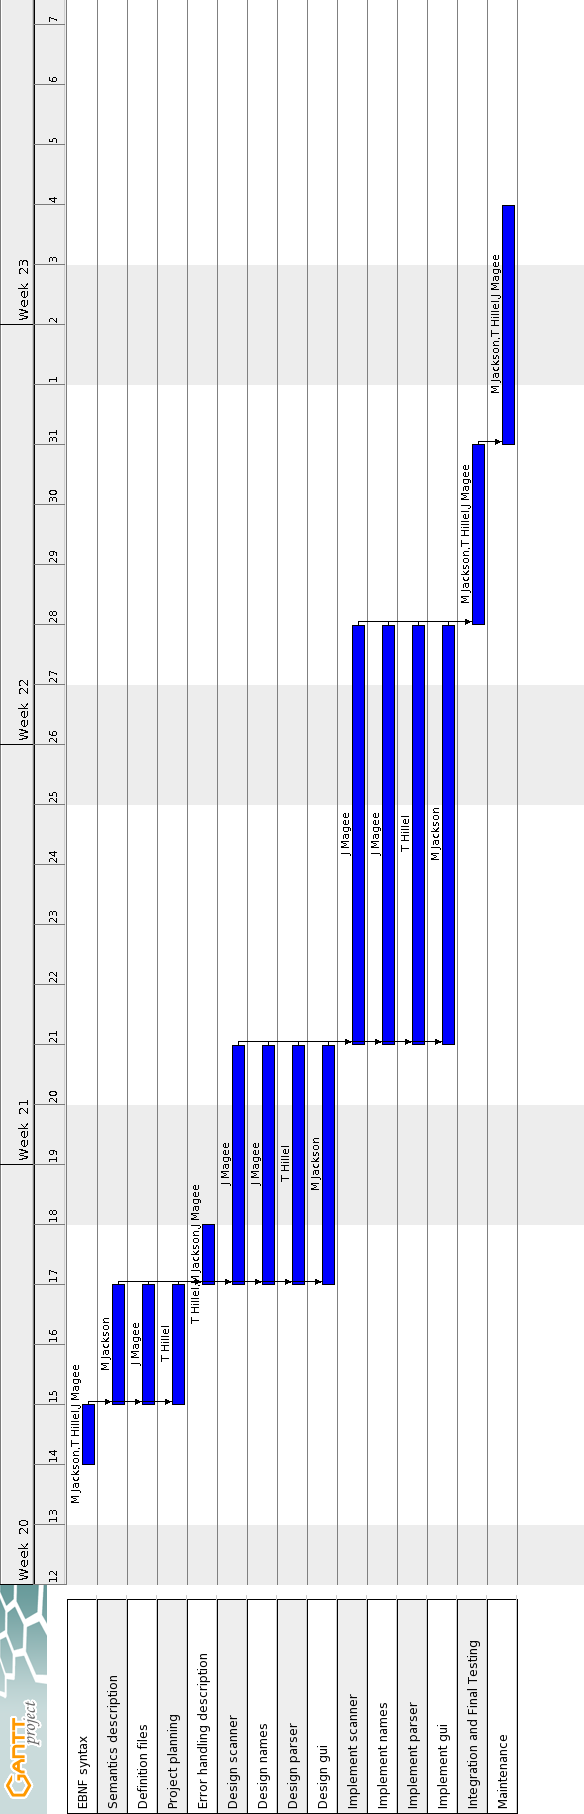
\includegraphics[height=.75\textheight]{../../report1/Gantt-Chart.png}
 \caption{Gantt chart showing our development cycle}
 \label{fig:ganttchart}
\end{figure}
\pagebreak

\end{document}